\chapter{Flots de liens: extension temporelle des graphes}
\minitoc
\label{chap:def_flot}

\section{Définition}
\label{sec:definition}

Nous avons décrit rapidement le formalisme de flot de liens dans le chapitre précédent.
Nous nous attachons maintenant à définir plus formellement les flots de liens et quelques notions utilisées dans le reste de cette thèse.
Un flot de liens est défini par un triplet $L=(T,V,E)$ où $T=[\alpha, \omega]$ est un intervalle de temps, $V$ un ensemble de $n$ n\oe uds et $E\subseteq T\times T \times V \times V$ un ensemble de $m$ liens.
Les liens de $E$ sont des quadruplets $(b,e,u,v)$, signifiant que la paire de n\oe uds $(u, v)$ est connectée sur l'intervalle $[b,e] \subseteq [\alpha,\omega]$.
Nous dénotons la durée du flot par $\bar{L}=\omega-\alpha$.
De manière analogue, la durée d'un lien $l=(b,e,u,v) \in E$ est notée   $\bar{l}=e-b$.
$\beta(E)= min_{(b,e,u,v) \in E} (b)$ et $\psi(E)= max_{(b,e,u,v) \in E} (e)$ sont respectivement l'apparition du premier lien et la disparition du dernier lien dans le flot de liens.

Nous considérons les flots de liens non orientés et sans boucle, \emph{i.e.}$(b,e,u,v)=(b,e,v,u)$ et $u \neq v$.
Enfin de manière analogue aux graphes et les multigraphes, nous définissons les flots de liens simples.
Un flot de liens est simple si pour tout $l_1=(b,e,u,v) \in E$ et $l_2=(b',e',u, v) \in E$, $[b,e]\cap [b', e'] = \emptyset$ si $l_1 \neq l_2$.
Dans les graphes, il est possible de transformer un multigraphe en graphe simple.
Nous définissons également cette opération que nous nommons simplification: $\sigma(L)$.
Afin de définir la simplification, nous nous aidons de la fonction de présence $\zeta_{L}(u,v,t)$ d'un flot de liens qui est égale à $1$ si au moins un lien existe dans le flot $L$ entre $u$ et $v$ à l'instant $t$ et $0$ sinon
$L'=(T',V',E')= \sigma(L)$ est la simplification de $L=(T,V,E)$ si et seulement si $L'$ est simple, $T'=T$, $V'=V$ et si $\forall u,v \in V,\ \forall t\in T, \zeta_{L}(u,v,t)= \zeta_{L'}(u,v,t)$.

Il est parfois nécessaire d'augmenter la durée des liens.
C'est notamment utile lorsque les liens sont de la forme $(t,t,u,v)$, ce qui est le cas lorsqu'on étudie des envoies de courriels par exemple.
Nous notons $\xi(L,\Delta)=L'$ le fait d'augmenté de $\Delta$ la durée de chaque lien.
Il y a plusieurs moyen d'augmenter de $\Delta$ un intervalle $[b,e]$.
Nous considérons l'ajout symétrique c'est à dire qu'un intervalle $[b,e]$ est transformé en l'intervalle $[b-\Delta/2,e+\Delta/2]$.

Enfin, il est parfois intéressant d'agréger l'information temporelle pour créer un graphe statique.
Un graphe $G=(V,E')=G(L)$ est le graphe agrégé d'un flot de liens si $\forall (u,v) \in E',\ \exists b,e \in T$ tel que $(b,e,u,v) \in E$.


%Une fois défini les flots de liens, nous pouvons commencer à définir différentes opérations pour les analyser.


\section{Sous-flots}
Dans les graphes, il existe la notion de sous graphes que nous étendons également aux flots de liens.
Un flot de liens $L'$ est un sous-flot de $L$, $L' \subset L$, si  $\forall u,v \in V,\ \forall t\in T, \zeta_{L'}(u,v,t) \leq \zeta_{L}(u,v,t)$.
Cette notion est en particulier utile pour définir des sous-flots induits par différent éléments.
Nous illustrons ces notions dans les figure~\ref{fig:exemple_sous_flot1} \ref{fig:exemple_sous_flot1} et \ref{fig:exemple_sous_flot1} avec le flot initial dans la figure~\ref{fig:exemple_sous_flot_init}.
 
Nous définissons $L(E')$ , le sous-flot de $L$ inuit par un ensemble de liens $E' \subset E$: $L(E')=([\beta(E'),\psi(E'),V(E'),E'])$.

 
Nous définissons $L(S)$ , le sous-flot de $L$ induit par un ensemble de paires n\oe uds $S \in V^ 2$: $L(S)$: $L(S)=([\beta(E'),\psi(E')],V',E')$ avec $E'= \{(b,e,u,v) \in E, (u,v) \in S\}$.
Par convention, on note $L(v)= L(\{v\}\times V)$, le sous-flot induit par un n\oe ud.
Un exemple de sous-flot induit par un n\oe ud est dans la figure~\ref{fig:exemple_sous_flot1}.


Enfin, nous définissons $L_{t..t'}$, le sous-flot de $L$ induit par l'intervalle de temps $[t,t'] \subset [\alpha, \omega]$: $L_{t..t'}=([t, t'], V,E')$ avec $E'= \{(b',e',u,v),\ \exists (b,e,u,v) \in E,\ b'= max(b,t),\ e'=min(e,t')\}$.
Il est également possible de définir $L_{t..t'}$ via la fonction de présence: $\forall u,v \in V,\ \forall x \in [t,t']\  \zeta_{L_{t..t'}}(u,v,x) = \zeta_{L}(u,v,x)$.
Un exemple de sous-flot induit par un intervalle de temps est présenté dans la figure~\ref{fig:exemple_sous_flot2}.
Il est intéressant de noter que le sous-flot $L_t..t$ est équivalent au graphe statique à l'instant $t$,  que nous notons $G(L_t)$.


\begin{figure}[]
\centering
	\begin{subfigure}{0.25\linewidth}
		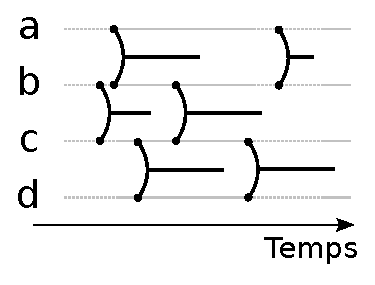
\includegraphics[width=\linewidth]{img/Intro/sous_flots.eps}\hfill
		\caption{Flot de liens initial $L$}
		\label{fig:exemple_sous_flot_init}	
	\end{subfigure}\hspace{0.1\linewidth}
	\begin{subfigure}{0.25\linewidth}
		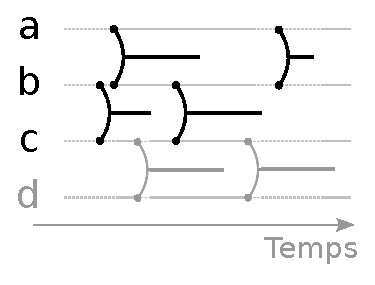
\includegraphics[width=\linewidth]{img/Intro/sous_flots1.eps}\hfill
		\caption{Sous-flot induits par des n\oe uds: $L(b)$}	
		\label{fig:exemple_sous_flot1}	
	\end{subfigure}\hspace{0.1\linewidth}
	\begin{subfigure}{0.25\linewidth}
		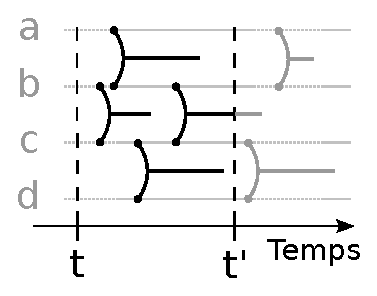
\includegraphics[width=\linewidth]{img/Intro/sous_flots2.eps}\hfill
		\caption{Sous-flot induits par le temps:  $L_{t..t}$}
		\label{fig:exemple_sous_flot2}	
	\end{subfigure}
	\caption{Exemple de différents sous-flots, (B) et (C), du flot initial en (A). Les liens en noirs sont les liens sélectionnés dans le sous-flot. }
\label{fig:exemple_sous_flot}
\end{figure}
Enfin, il est aussi possible de combiner ces notions.
Par exemple avec $V' \subset V$, $L_{\alpha'..\omega'}(V'\,^2)$ est le sous-flot correspondant aux liens entre les n\oe uds de $V'$ sur l'intervalle $[\alpha', \omega']$.

\bigskip

La construction d'un sous-flot induit par un ensemble de paires de n\oe uds peut être faite de manière linéaire au nombre de liens dans le sous-flot.
Pour un ensemble de paires de n\oe uds $S= V_1 \times V_2$, il suffit d'itérer sur l'ensemble des liens qui sont reliés aux n\oe uds de $V_1$ et de vérifier que l'autre n\oe ud du lien appartienne à $V_2$ ce qui se fait en $O(log(|V_2|))$ pour chaque lien.
Cela peut être fait rapidement si chaque n\oe ud a la connaissance des ces liens.
Il faut tout de fois distinguer le cas où $S= V_1 \times V$ car il n'est alors pas nécessaire de faire la vérification d'appartenance à $V$.

Pour l'intervalle de temps, la situation est plus compliquée car il n'est pas facile de connaitre l'ensemble des liens existent à un insant donné.
Il est uniquement possible de les trier par ordre d'apparition ou de disparition.
Il n'y a pas d'ordre total sur la présence qui permettrait de considérer uniquement les liens appartenant au sous-flot.
Pour qu'un lien, $l= (b,e,u,v)$ appartienne au sous-flot temporel sur $[t,t']$, il doit remplir une des ces conditions, qui ne sont pas exclusives:
\begin{enumerate}
\item $t \leq b \leq t'$ le lien commence dans l'intervalle $[t,t']$.
\item $t \leq e \leq t'$ le lien fini dans l'intervalle $[t,t']$.
\item $ b \leq t \, \wedge \, t' \leq e$ le lien couvre tout l'intervalle $[t,t']$.
\end{enumerate}

Avec ces conditions, on peut tirer deux conclusions.
Pour qu'un lien $l=(b,e,u,v)$ puisse appartenir au sous-flot, il est nécessaire que $e \geq t$.
Il n'est donc pas nécessaire de considérer les liens ayant un temps de fin inférieur à $t$.
De manière analogue, il n'est pas nécessaire de considérer les liens ayant un temps de début supérieur $t'$.
Cependant ces deux conditions ne peuvent pas être combinées pour restreindre l'espace de recherche.
Une manière de construire le sous-flot temporel est d'itérer sur tous les liens dans l'ordre temporel d'apparition et d'arrêter le parcours dès qu'un lien a un temps de début supérieur à $t'$.
Il faut cependant tester l'appartenance de chaque lien parcouru.
De manière analogue, il set possible d'itérer sur les liens dans l'ordre inverse de disparition des liens et de s'arrêter dès qu'un lien a une temps de fin inférieur à $t$.


Dans le pire des cas, ces méthodes sont donc linéaire sur le nombre total de liens dans le flot et non dans le sous-flot comme précédemment.
Il n'y a alors que deux optimisations possibles.
il est possible de choisir le sens du parcours si les deux ordres sont disponibles.
Si la plus longue durée de liens,$\bar{l}_{max}$, est connue, alors il est possible de commencer la recherche à partir du premier lien respectant $b+\bar{l}_{max} \geq t$.



\section{Degré et densité}
\label{sec:def_densite}
Nous avons défini des outils pour manipuler et extraire un flot de liens.
Nous nous intéressons maintenant à étendre quelques notions de connexités qui existe dans le graphe, en particulier le degré et la densité.


Il est assez trivial de définir le degré temporel d'un n\oe ud $u$ de la manière suivante:
\begin{equation}
d(t,u)=d_t(u)= |L_t(u)|= \sum_{v \in V} \zeta_{L}(u,v,t).
\end{equation}
Le degré temporel n'est alors pas une simple valeur mais une fonction qui dépend du temps.
Comme les liens apparaissent et disparaissent de manière instantanée, la fonction de degré est une fonction constante par morceaux.
Un exemple de degré temporel est présenté dans la figure~\ref{fig:exemple_degre}.

\begin{figure}
\centering
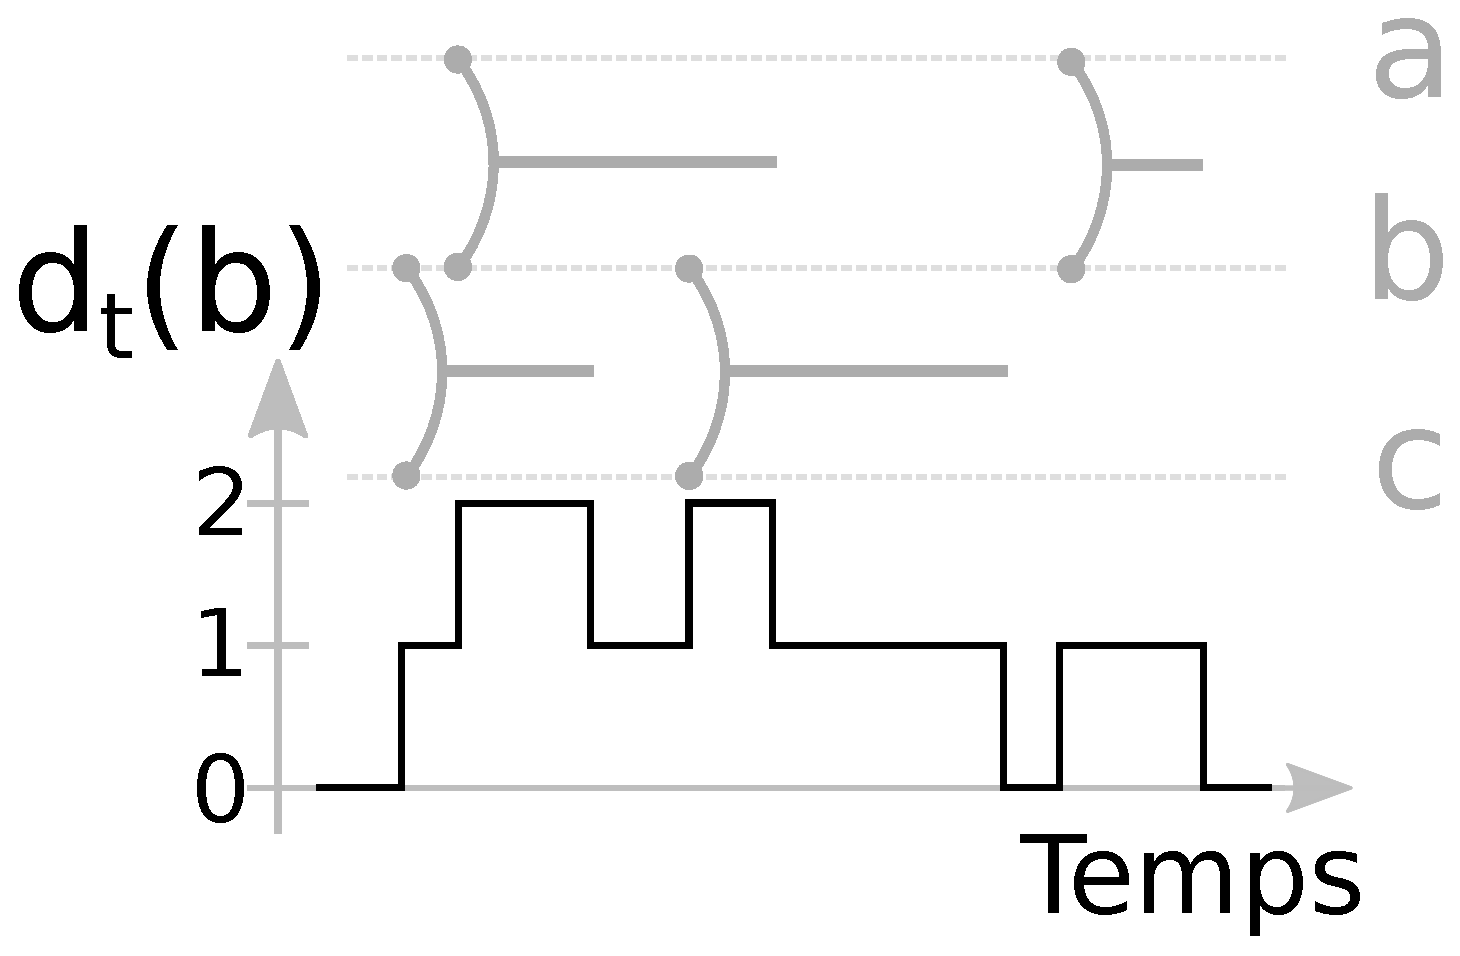
\includegraphics[width=0.5\linewidth]{img/Intro/degre2.eps}
\caption{Degré temporel du n\oe ud $b$ dans le flot de liens dans la figure~\ref{fig:exemple_sous_flot_init} qui est également rappelé en grisé dans cette figure.
}
\label{fig:exemple_degre}
\end{figure}

De manière analogue aux graphes, il est également possible de définir le degré temporel d'un ensemble de n\oe uds ou d'un ensemble de liens:

\begin{equation}
d_t(V')= \sum_{v \in V'} d_t(v) = 2 |L_{t}(V'^2)| = 2|\{(b,e,u,v) \in E,\ u,v \in V',\ b \leq t \leq e\}|\,,
\end{equation}

\begin{equation}
d_t(E')=2|L_{t}(E')|= 2|\{(b,e,u,v) \in E',\ b \leq t \leq e\}|\,.
\end{equation}

Avec ces définitions, il est aussi possible définir les notions de degré temporel interne, $d_t^{in}$, et externe $d_t^{out}$.
Les degrés temporels d'un n\oe uds, d'un ensemble de n\oe uds ou de liens peuvent se calculer rapidement.
Pour ce faire, il faut d'abord transformer les liens $(b,e,u,v)$ en une suite de modifications de la forme $(b,u,v,+1)$ et $(e,u,v,-1)$ ce qui a une complexité en $O(m)$.
Une fois cette liste créée, il suffit d'ordonner ces modifications dans l'ordre temporelle, $O(2mlog(2m))$, puis d'itérer sur l'ensemble des modification en sommant au fur et à mesure les apparitions et disparitions de lien, $O(2m)$.
\bigskip

Les degrés sont des fonctions du temps mais il est souvent intéressant de regarder la valeur moyenne du degré:
\begin{equation}
d_{t..t'}(u)=\dfrac{1}{t'-t}  \int_{t}^{t'}d(u,t) dt = \sum_{l \in L_{t..t'}(u)} \dfrac{\bar{l}}{t'-t} \, .
\label{eq:deg_moyen}
\end{equation}

Lorsque cela n'est pas ambigu, nous notons $d_{\alpha..\omega}(u) = d(u)$.
Il est intéressant de noter dans cette formulation que si tout les liens durent tout au long du flot de liens alors le degré dans le graphe agrégé et le degré moyen dans le flot de liens sont égaux, c'est-à-dire  $d_{\alpha..\omega}(u) = d_{G(L)}(u), \forall u \in V$.

\'A partir du degré, il est possible de définir beaucoup de notions différentes et notamment la densité.
Pour rappel, la densité dans un graphe est définie par $\delta(G)=2m/(n(n-1))=d(V)/n(n-1)$ et est égale à la probabilité qu'il existe un lien entre 2 n\oe uds.
Si l'on transpose l'idée au formalisme de flot de liens, la densité dans un flot de liens est la probabilité qu'il existe un lien entre 2 n\oe uds à un instant donné aléatoire.
Cela se traduit par la formule suivante:
\begin{equation}
\delta(L)= \dfrac{2 \sum_{l \in E}\bar{l}}{n(n-1) (\omega-\alpha)}.
\end{equation}

Il se trouve que cette formulation est complètement équivalente à la densité moyenne des graphes $G(L_t)$:

\begin{equation*}
\dfrac{1}{\omega-\alpha} \int_{\alpha}^{\omega} \delta(G(L_t)) dt=
\dfrac{1}{\omega-\alpha} \int_{\alpha}^{\omega} \dfrac{d(t,V)}{(n-1)}dt=
 \dfrac{1}{\omega-\alpha} \int_{\alpha}^{\omega} \dfrac{\sum_{u \in V} d(t,u)}{n(n-1)}dt = 
 \dfrac{\int_{\alpha}^{\omega} \sum_{u \in V} d(t,u)dt}{n(n-1)(\omega-\alpha)} 
 \end{equation*}

 \begin{equation*}
 =
\dfrac{\sum_{u \in V} \int_{\alpha}^{\omega}d(t,u)dt}{n(n-1)(\omega-\alpha)} =
\dfrac{\sum_{u \in V} \sum_{l \in L_{\alpha..\omega}(u)} \bar{l}}{n(n-1)(\omega-\alpha)} =
\dfrac{\sum_{u \in V} \sum_{l \in L_(u)} \bar{l}}{n(n-1)(\omega-\alpha)}=
\dfrac{2\sum_{l \in E}\bar{l}}{n(n-1) (\omega-\alpha)} .
\end{equation*}

Pour arriver à ce résultat, nous utilisons la relation entre degré temporel moyen et somme des durées de l'équation~\ref{eq:deg_moyen} et le fait que la somme des degrés soit égale à deux fois le nombre de liens.

La notion de densité que nous avons définie est donc cohérente avec notre notion de degré et traduit le même concept que dans les graphes.
Ainsi, la densité dans les flots de liens est aussi comprise entre à $0$ et $1$.
Enfin, cette formulation de densité est une généralisation de la densité proposée par Viard~\emph{et al.}~\cite{Viard2014a} qui ne considérait que les liens sans durée.

Le calcul de la densité d'un flot est linéaire en le nombre de liens car elle est dépendante du calcul de $d_{\alpha..\omega}(V)$  qui est fait de manière linéaire.
\clearpage
\section{Liste des notations pour les flots de liens}
\begin{table}[h]
	\centering
	\begin{tabular}{|c|c|}
	\hline Symbole & description \\
	\hline $L$ & Flot de liens \\ 
	$T$ & intervalle de temps  \\
	$V$ & ensemble de n\oe uds\\
	$E$ & ensemble de liens: $(b,e,u,v)$ \\
	$n$ & nombre de n\oe uds  \\
	$|L|,|E|$ & nombre de liens dans le flot \\
	$\beta(E)$ & temps d'apparition du premier lien\\
	$\psi(E)$ & temps de disparition du dernier lien\\
	$\xi(L,\Delta)$ & Flot de liens où chaque lien dure $\Delta$\\
	$\sigma(L)$ & Simplification du flot de liens $L$\\
	$L(V'^2)$ & sous-flot induits par les n\oe uds de $V'$ \\
	$L_{t..t'}$ & sous-flot induits par l'intervalle $[t,t']$ \\
	$d_t(v)$ & degré de $v$ à l'instant $t$\\
	$d_t(V)$ & Somme des degrés des n\oe uds dans $V$ à l'instant $t$\\
	$d_{t..t'}(v)$ & degré moyen de $v$ sur $[t,t']$\\
	$d(v)$ & degré moyen $v$ sur $T$\\
	$\delta(L)$ & densité du flot\\
%	$\delta_{\Delta}(L)$ & densité du flot où chaque lien dure $\Delta$\\
	\hline
	\end{tabular} 
		\caption{Liste des notations pour les flots de liens}
\end{table}

\section{Manipulation concrète des flots de liens}

Nous avons défini formellement quelques notions pour les flots de liens.
Afin de manipuler ces notions simplement, nous avons mis en place une librairie capable de les calculer simplement.
Le but est de fournir une implémentation généraliste qui soit simple d'accès.
Ainsi, il sera possible à n'importe qui de calculer ces notions.
La démarche, bien que beaucoup plu modeste, est similaire à ce qui est fait avec les graphes et networkx\,\footnote{\url{https://networkx.github.io/}}.

L'implémentation est en \emph{C++} pour être rapide avec un export en \emph{python} pour faciliter l'utilisation.
Le code de cette implémentation est ligne\,\footnote{\url{XXX}}\note{A Mettre} et la documentation également\,\footnote{\url{XXX}}\note{A Mettre}.
Il est par exemple possible avec la librairie de lire un flot de liens et de calculer la densité moyenne d'un sous-ensemble de n\oe uds sur un intervalle arbitraire.
Comme le but de cette librairie est d'être généraliste, l'implémentation n'est pas optimisée en espace pour un calcul spécifique.
Ainsi il est aisé d'étendre la librairie en écrivant un nouveau calcul.
 

Un intérêt de cette implémentation est de permettre, en python, la génération de visualisation\,\footnote{Pour  l'instant, uniquement un export en svg est possible.}, voir le dessin dans la figure~\ref{fig:exemple_Flot_de_liens_lib}.
Parmi les possibilités offertes par la visualisation, il est possible de n'afficher qu'une partie des n\oe uds ou de ne garder qu'un sous intervalle de temps.
De plus, il est possible de choisir la couleur des liens de manière manuelle ou en fonction d'une partition de liens.

\begin{figure}
\centering
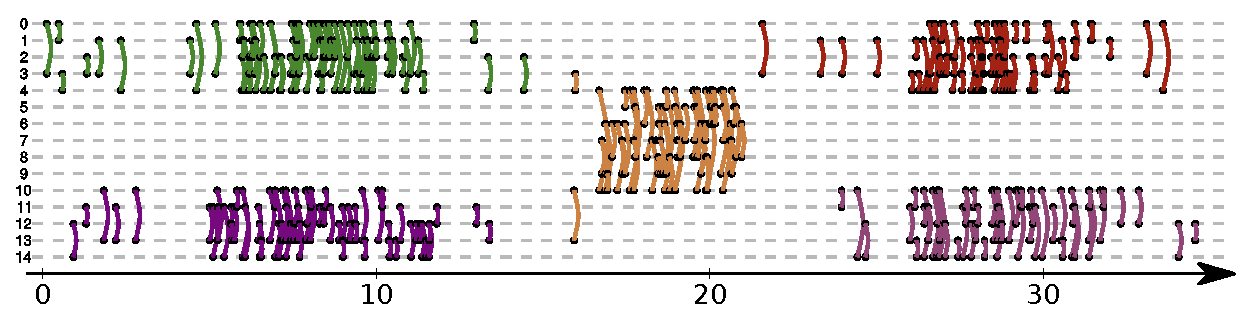
\includegraphics[width=\linewidth]{img/Intro/Dessin_Flot.eps}
\caption{Flot de lien entre $6$ n\oe ds, représenté sur l'axe des ordonées, au cours du temps représenté sur l'axe des abscisses.
Dans l'exemple, il existe un lien entre $a$ et $b$ durant l'intervalle $[4,6]$.
}
\label{fig:exemple_Flot_de_liens_lib}
\end{figure}

La lisibilité de ce genre de visualisation est très dépendant de l'ordre attribué aux n\oe uds sur l'axes des ordonnées.
C'est pourquoi avec notre outil, il est également possible de fixé un ordre arbitraire.
Comme il peut être fastidieux d'écrire un ordre, nous avons implémenté un algorithme rudimentaire pour améliorer l'ordonnancement des n\oe uds dans la visualisation.
Avant de pouvoir améliorer une visualisation, il est nécessaire de pouvoir quantifier la complexité de la visualisation actuel.
Empiriquement, on se rend vite compte que ce sont les long traits verticaux qui rende pénible la lecture et qu'il faut limiter.

C'est pourquoi nous décidons d'évaluer une ordonnancement en fonction de la somme des longueurs des traits représentant les liens.
Avec la fonction d'ordre $Ordre: V \longmapsto \mathbb{N}$, trouver le meilleur ordonnancement se résume à résoudre:

\begin{equation}
 Ordre* = \argmin_{Ordre}  \sum_{(b,e,u,v) \in E} |Ordre(u)- Ordre(v)|
\end{equation}

Malheureusement, trouver l'optimum ne semble pas trivial et il n'est pas envisageable de tester l'ensemble des ordre.
C'est pourquoi, nous utilisons un algorithme probabiliste qui teste certain nombre de permutations aléatoire.
Une permutation est appliquée si elle améliore l'évaluation de la visualisation.
Il s'agit bien sur d'une première approche qu'il est possible d'améliorer.

Une piste possible pour améliorer cette approche naïve serait la construction d'un ordre potentiellement proche de l'optimum.
Pour y arriver, il serait intéressant de placer côte à côte les n\oe uds qui partagent le plus de liens et ainsi construire itérativement une première solution.